


% CHAPTER:  1
% (Note: cannot have a footnote on a word within the \chapter{} construct, it does not work)
\newcommand{\s}{$_{\rm s}$}
\newcommand{\kms}{km~s$^{-1}$}
\newcommand{\msun}{{\it M}$_{\odot}$}
\newcommand{\lsun}{{\it L}$_{\odot}$}
\newcommand{\mear}{{\it M}$_{\oplus}$}
\newcommand{\etal}{{\it et al.}}
\newcommand{\ie}{{\it i.e.}}
\newcommand{\eg}{{\it e.g.}}
\newcommand{\be}{\begin{equation}}
\newcommand{\ee}{\end{equation}}
\newcommand{\magarc}{{\rm mag\,arcsec$^{-2}$}}
\newcommand{\MK}{{{\rm M}_{\rm ext,K}-5\log h}}
\newcommand{\ri}{{$r_{21}$}}
\newcommand{\ra}{$R_A$}
\newcommand{\vobs}{{v_{\rm obs}}}
\newcommand{\kmsMpc}{km~s$^{-1}$ Mpc$^{-1}$}
\newcommand{\h}{$h_{70}$}
\newcommand{\vpec}{v_{\rm pec}}
\newcommand{\like}{{\mathcal L}}
\newcommand{\vs}{\vspace*{5pt}}
\newcommand{\continued}{ (Continued)}

\newcommand{\ferengi}{\textsc{ferengi}}
\newcommand{\hst}{\textit{HST}}
\newcommand{\hubble}{\textit{Hubble Space Telescope}}
\newcommand{\subaru}{\textit{Subaru}}
\newcommand{\sextractor}{\textsc{SExtractor}}
\newcommand{\galapagos}{\textsc{Galapagos}}
\newcommand{\galfit}{\textsc{GALFIT}}
\newcommand{\gimtwod}{\textsc{GIM2D}}
\newcommand{\sersic}{S\'{e}rsic}






% Galaxy Zoo
\newcommand{\ffeatures}{$f_{\rm features}$}
\newcommand{\ffeaturesz}{$f_{\mathrm{features,}z}$}
\newcommand{\ffeaturesrest}{$f_{\mathrm{features,}z=0.3}$}
\newcommand{\ffeaturesdebiased}{$f_{\mathrm{features,debiased}}$}
\newcommand{\fbest}{$f_{\mathrm{features,best}}$}
\newcommand{\fodd}{$f_{\mathrm{odd}}$}
\newcommand{\fbar}{$f_{\mathrm{bar}}$}
\newcommand{\fclumpy}{$f_{\mathrm{clumpy}}$}
\newcommand{\fsmooth}{$f_{\rm smooth}$}
\newcommand{\fartifact}{$f_{\rm artifact}$}

\newcommand{\fHI}{f_{\rm HI}}
\newcommand{\zsim}{$z_{\mathrm{sim}}$}

% Bands

\newcommand{\Bband}{$B_{435W}$}
\newcommand{\Vband}{$V_{606W}$}
\newcommand{\iband}{$i_{775W}$}
\newcommand{\Iband}{$I_{814W}$}
\newcommand{\zband}{$z_{850LP}$}

% GZH subsamples

\newcommand{\main}{\texttt{main}}
\newcommand{\faded}{\texttt{faded}}
\newcommand{\recolored}{\texttt{recoloured}}
\newcommand{\goods}{\texttt{goods-shallow}}
\newcommand{\stripe}{\texttt{stripe-82-single}}
\newcommand{\coadd}{\texttt{stripe-82-coadd}}
\newcommand{\redshifted}{\texttt{redshifted}}
\newcommand{\simagn}{\texttt{simulated-agn}}



\chapter{FERENGI: debiasing beyond the local Universe}
\label{chap:ferengi}
\begin{quote}
\emph{ Portions of this chapter has been published in the Montly Notices of the Royal Astronomical Society with the following bibiliographic reference:  Willett, K. W., Galloway, M. A., et al., 2015 ?}\\
\end{quote}
\section{Intro}
\label{sec:ferengi_Intro}
%% motivate importance of f_features in selecting morphological samples for population studies, and introduce the bias induced in the measurement as a function of redshift 

The GZ vote fraction \ffeatures{} plays a crucial role in the majority of science cases that use Galaxy Zoo classifications. It represents the fraction of users who answered ``feature or disk'' to the first question in the decision tree, and is used to distinguish elliptical/spheroidal galaxies from those with features. Many studies aim to measure the popluation of galaxies exhibiting certain features such as bars \citep{Masters2010,Masters2012,Melvin2014,Simmons2014,Cheung2015,Kruk2017}, spiral arms \citep{Willett2015,Hart2017}, or bulges \citep{Skibba2012,Simmons2012}, among others. In each of these, \ffeatures{} is necessary for creating the sample of galaxies which could potentially contain the feature in question. This is typically acheived by setting a cut, such that all galaxies with \ffeatures{} greater than that threshold are considered to be candidates for that study.

While \ffeatures{} is not a true probability, the measurement is intended to be consistent among all galaxies; that is, two galaxies with similar \ffeatures{} values should have similar likelihoods of being featured (or not featured). This has been shown to be true at low redshift by comparing the \ffeatures values to expert classifications \citep{Willett2013}; there is a strong correlation between this vote fraction and whether the galaxy was expertly classified as a disk or an elliptical.    

For distant galaxies, however, we observe that \ffeatures{} is not consistant with nearby galaxies. As galaxies are observed at higher redshift, the images are inherently less resolved, and smaller features are more difficult to identify. This causes in a decrease in \ffeatures{} than what would be expected if the galaxy had been observed at $z=0$. Figure~\ref{fig:features_example} shows this effect: although each of the five galaxies displayed appear to be discs with features, the fraction of users who identify the images in this way decreases with increasing redshift, as the finer features in each, while still present, become more difficult to resolve. Therefore, two intrinsically identical galaxies, but imaged at different redshifts, may have small to drastic differences in their \ffeatures{} measurements. In order to keep \ffeatures{} a value correlated with the likelihood of having features that is consistent for \emph{all} galaxies, this bias must be corrected.

\begin{figure}
\centering
\includegraphics[width=\textwidth]{figures/features_example.pdf}
\label{fig:features_example}
\caption{Example of the redshift-induced bias in \ffeatures{}. Five images of disc galaxies from the GZH dataset are shown in order of increasing redshift, from left to right. Above each galaxy is its redshift and below is its \ffeatures{} vote fraction. Although all galaxies appear to be discs with features, the vote fraction decreases steadily as redshift increases, as the details in each image become more difficult to distinguish.}
\end{figure} 

A method for correcting redshift bias in the GZ vote fractions was developed and implemented in early Galaxy Zoo projects GZ1 \citep{Lintott2009} and GZ2 \citep{Willett2013}, which both contained nearby ($z<0.2$) galaxies imaged by SDSS. A correction factor to the classification fractions measured at the higher redshifts was applied by matching the mean vote fractions of those at the lowest redshift. This technique was valid under the assumption that, within this redshift range, there would be no cosmological evolution of galaxies, and therefore any change in the mean vote fraction for any morphology with redshift was purely due to this observational bias, and not due to a genuine difference in morphological populations. For a full description, see Chapter~\ref{chap:methodology}. 

In GZH, the redshift range is large enough that cosmological evolution of the morphologies of galaxies is expected, and therefore the previous method of correcting redshift-bias will not work. Instead, a new method was developed of measuring the change in \ffeatures{} as a function of redshift using a set of simulated \ferengi{} images of galaxies, described in the next section. These images have been classified by volunteers in Galaxy Zoo in the same way as the GZH sample. This chapter will describe how a correction factor for \ffeatures{} is measured using these data as a function of redshift at fixed surface brightness, and subsequently used to debias to the GZH sample. 

\subsection{The FERENGI code}
\label{sec:ferengicode}
The Full and Efficient Redshifting of Ensembles of Nearby Galaxy Images code (FERENGI, \citet{Barden2008}) is an IDL procedure that generates simulated images of nearby galaxies viewed at higher redshifts, taking into account cosmological effects such as surface brightness dimming and bandpass shifting. Artificially redshifted samples of galaxies, for which the intrinsic morphologies are already known from low-redshift observations, are useful for studying the imact these effects have on observed galaxy morphologies. For Galaxy Zoo, such images are particularly useful for measuring the effects of redshift on the volunteer classifications. Through classifications made on a set of artificially redshifted galaxies, any dependence they might have as a function of redshift can be measured, allowing a correction to be applied to classifications on images of real, high-redshift galaxies. The details of this type of debiasing technique will be described in Section~\ref{sec:ferengidebiasing}. This section will first provide a breif summary of how the FERENGI code performs the artificial redshifting.

To create realistic images that mimic the seeing and resolution of HST ACS, the FERENGI redshifting procedure consists of three primary steps (explained in detail in \citet{Barden2008}, but here a simplified outline):

\textbf{i: Modify angular size and surface brightness}

FERENGI first rescales the input image by computing the angular size transformation of the galaxy from its input redshift $z_{i}$ to output reshift $z_{o}$. The angular size $a$ of a distant object is proportional to $a \propto d/(1+z)^2$ (using tan($a$)=$a$ for small angles), where $d$ is the luminosity distance to the object. In units of pixels, the transformation from input angular size $n_{i}$ to output $n_{o}$ can be expressed as:

\begin{equation}
\frac{n_{o}}{n_{i}}= \frac{d_{i}/(1+z_{i})^2}{d_{o}/(1+z_{o})^2} \frac{p_{i}}{p_{o}} 
\label{eqn:ferengi_rebinning}
\end{equation}

with an input pixel scale $p_{i}$ (in this thesis $p_{i}=0.396''$/pix corresponding to SDSS) and $p_{o}$ (0.03''/pix, corresponding to ACS). From here a transformation between the observed fluxes is computed, assuming the absolute magnitude is conserved at both redshifts. 

FERENGI also offers an option to apply an evolutionary correction to the absolute magnitude, which is helpful for a fair comparison of real and artificial high redshift morphologies. Artificially redshifted galaxies will appear much dimmer than their low redshift counterparts if absolute magnitude is conserved.  Since galaxies intrinsically tend to be brighter at high redshift, visual classification of real galaxies cannot be compared as accurately to dimmer, simulated galaxies. To brighten galaxies in a similar way to real galaxies, a magnitude correction $e$ can be input using a linear function:

\begin{equation}
M_{evo} = e \times z + M
\label{eqn:ferengievolution}
\end{equation}

where $e$ represents the magnitude difference between two redshifts separated by $\Delta z=1$. 

\textbf{ii: Account for bandpass shifting} 

As a consequence of cosmological expansion, the flux from a source measured using a broadband filter will not, in general, perfectly correspond to the rest-frame flux emitted at the target wavelength range of the filter. Rather, since observed wavelengths are redder than emitted wavelengths as a function of redshift ($\lambda_{obs}=\lambda_{rest-frame}(1+z)$), filters will tend to pick up light that is bluer (in the galaxy's rest-frame) than its target wavelength; this effect is known as \emph{bandpass shifting}. In order to produce fluxes that mimic those measured by ACS at high redshifts, FERENGI simulates the bandpass shifting effects by applying a correction to the output flux calculated via the IDL routine \textsc{kcorrect}, which incorporates spectral template models from \citet{Bruzual2003}, to measure the expected shifts in flux for a given output filter.   

\textbf{iii: Point Spread Function and noise}

In order to best mimic the HST ACS resolution, the image is then convolved with a PSF created to be as close as possible in shape and width to the ACS PSF. This is done by deconvolving a typical ACS PSF with the input SDSS PSF for each galaxy. This technique works well in general but has limitations - mainly, the widths of the in- and output PSFs must be sufficiently different. If they are comparable, the convolving function can become too narrow. In these cases, the image will be introduced to noise which results in ringing patterns and other oddities (examples of images with this effect are shown in Section~\ref{ssec:ferengi2sample}). Since the difference in PSF widths increases with redshift, this imposes a minimum redshift at which FERENGI can successfuly create images for any given galaxy (discussed more in Section~\ref{sec:ferengi1sample}). Last, Poissonian noise is added to each pixel.



\section{The FERENGI sample}
\label{sec:ferengi1sample}

To generate an artificially redshifted sample of galaxies to be used in debiasing the Galaxy Zoo: Hubble catalog, a source sample was generated \footnote{The source sample for FERENGI was created by the Galaxy Zoo science team in 2012.}consisting of 288 galaxies from SDSS, all of which were previously classified in GZ2. These galaxies were chosen to span a wide range of morphologies, surface brightnesses, and redshifts. Seven morphological classes were considered: spiral galaxies, edge-on disks without a bulge, edge-on disks with a bulge, face-on disks with a bulge, galaxies with any features, galaxies undergoing mergers, and barred galaxies. For each of these categories, galaxies were chosen with from three ``strength'' bins, defined using the GZ2 vote fractions. Weak strengths were defined as having $f_{class}<0.2$, intermediate as $0.2<f_{class}<0.8$, and strong as $f_{class}>0.8$. In each strength bin, galaxies were also chosen to represent three different surface brightnesses: $\mu_{r}>21.5$, $20.5<\mu_{r}<21.5$, and $\mu_{r}<20.5$. Finally, from each morphological class, strength, and surface brightness bin, one galaxy was chosen for four redshift bins: $z<0.013$, $0.013<z<0.02$, $0.02<z<0.025$, and $z>0.025$, with the exception of the bar class, in which two galaxies were chosen for each redshift bin, doubling the sample size for that class.


The 288 SDSS galaxies were processed with the \ferengi{} code to mimic \hst~ imaging parameters \footnote{This work was done by Edmond Cheung, a Galaxy Zoo science team member.}, in order to ultimately measure and correct any redshift-dependant biases in the classifications of the real \hst~ images. I-814 and V-606 images, chosen to match the \hst~ ACS AEGIS imaging, were output for each subject at a range of redshifts and with a range of applied evolution factors. The range of simulated redshifts possible for any galaxy is dependent on the intrinsic redshift and size of the source galaxy, since the simulated images cannot be resampled at better angular resolution than the original SDSS data. This imposes a minimum simulated ``target'' redshift that can be achieved for each galaxy. For the lowest redshift bin in the source sample ($z<0.013$), galaxies could be redshifted the full range of $0.3<z<1.0$, in increments of $dz=0.1$. For the second lowest redshift bin, galaxies could only be redshifted in the range $0.5<z<1.0$, for the third, galaxies could be redshifted in the range $0.8<z<1.0$, and for the highest redshift bin, galaxies were only redshifted in \ferengi{} to $z=1.0$. Only galaxies which were redshifted the full range were considered in the debiasing procedure outlined in the next section~ (\ref{ssec:correctablesamples}), because the method calibrates galaxies to a low redshift of $z=0.3$, data for which is not available for galaxies in the remaining three redshift bins. Last, for each simulated redshift, a range of evolution factors was applied from $0<e<3$ in increments of $de=0.5$. 

The final \ferengi{} sample totals 6,624 simulated images which were classified as part of GZ4, using the same decision tree as used in GZH. The debiasing technique described next (Section~\ref{sec:ferengidebiasing}) used only the 4,446 images corresponding to the 72 galaxies which were redshifted the full $0.3<z<1.0$ range. Because the debiasing method takes into account surface brightness as a parameter, photometry was measured for all images using \sextractor{} \footnote{\sextractor{} measurements for the original \ferengi{} sample were done by Tom Melvin, a former Galaxy Zoo science team member.}. The mean surface brighness $\mu$ within effective radius ($R_{e}$) was calculated as:

\begin{equation}
\label{eqn:mu}
\mu = m + 2.5*\log_{10}{(2 \times (b/a) \times \pi R_e^2 )}
\end{equation}

where $m$ is {\tt MAG\_AUTO} in the \Iband{} band, $(b/a)$ is the galaxy
ellipticity (the profile RMS along the semi-major and -minor axes), and $R_e$
is the 50\% {\tt FLUX\_RADIUS} converted into arcsec.


 

% Figure - ferengi1 examples
\begin{figure}
\centering
\includegraphics[width=0.9\textwidth]{figures/example_ferengi.pdf}
\caption{Examples of two SDSS galaxies which have been run through the \ferengi{} code to produce simulated \hst~images. The measured value of \ffeatures{} from GZH for the images in each panel are (1) Top row: \ffeatures{} = (0.900, 0.625, 0.350, 0.350, 0.225) and (2) Bottom row: \ffeatures{} = (1.000, 0.875, 0.875, 0.625, 0.375).}
\label{fig:ferengi1_examples}
\end{figure}



\section{Measuring the dependence $z$ and $\mu$ on \ffeatures{} using the FERENGI classifications }
\label{sec:ferengidebiasing}
\subsection{Identifying ``correctable'' and ``lower limit'' samples.}
\label{ssec:correctablesamples}

The objective is to use the simulated data from \ferengi{} to predict, for a galaxy imaged at a redshift $z$, and with a measured \ffeaturesz{} value, what its \ffeatures{} value \emph{would have been} if it had been viewed at $z=0.3$. This predicted value is defined as the ``debiased' vote fraction \ffeaturesdebiased, and is calculated by applying a correction to the measured value of \ffeatures.

The amount that a galaxy's \ffeatures{} vote fraction must be corrected is assumed to primarily depend on the apparent size and brightness of the galaxy. As described in \ref{sec:ferengi_Intro}, these factors will affect the overall clarity of the image viewed by the GZ volunteers, which in turn affects the likelihood of being able to identify distinct feature. The apparent size and brightness are controlled by both instrinsic parameters (absolute size and luminosity), and extrinsic (distance to the galaxy). The change in \ffeatures{} then is measured as a function of redshift ($z$, an extrinsic freature, measuring distance to the galaxy), and surface brightness ($\mu$, an intrinsic feature, taking into account both brightness and size).   

Figure~\ref{fig:f_vs_f} shows the change in \ffeatures{} for \ferengi{} galaxies in bins of redshift and surface brightness. Points in each $z,\mu$ represent individual \ferengi{} galaxies. On the x-axis of each bin is the value of \ffeatures{} measured in that galaxy's $z=0.3$ image (the lowest redshift of the simulated images). On the y-axis of each bin is the value of \ffeatures{} measured in that galaxy's $z=z$ image, where $z$ corresponds to the redshift associated with that bin. As predicted, the value of \ffeatures{} measured at a higher redshift, $z$, is, in general, \emph{lower} than the value measured at lower redshift, $z=0.3$, \emph{for the same galaxy}. This effect is strongest as redshift increases (to the right in Figure~\ref{fig:f_vs_f}) and as surface brightness decreases (upwards in Figure ~\ref{fig:f_vs_f}). 

% Figure - big ass plot
\begin{figure}
\begin{center}
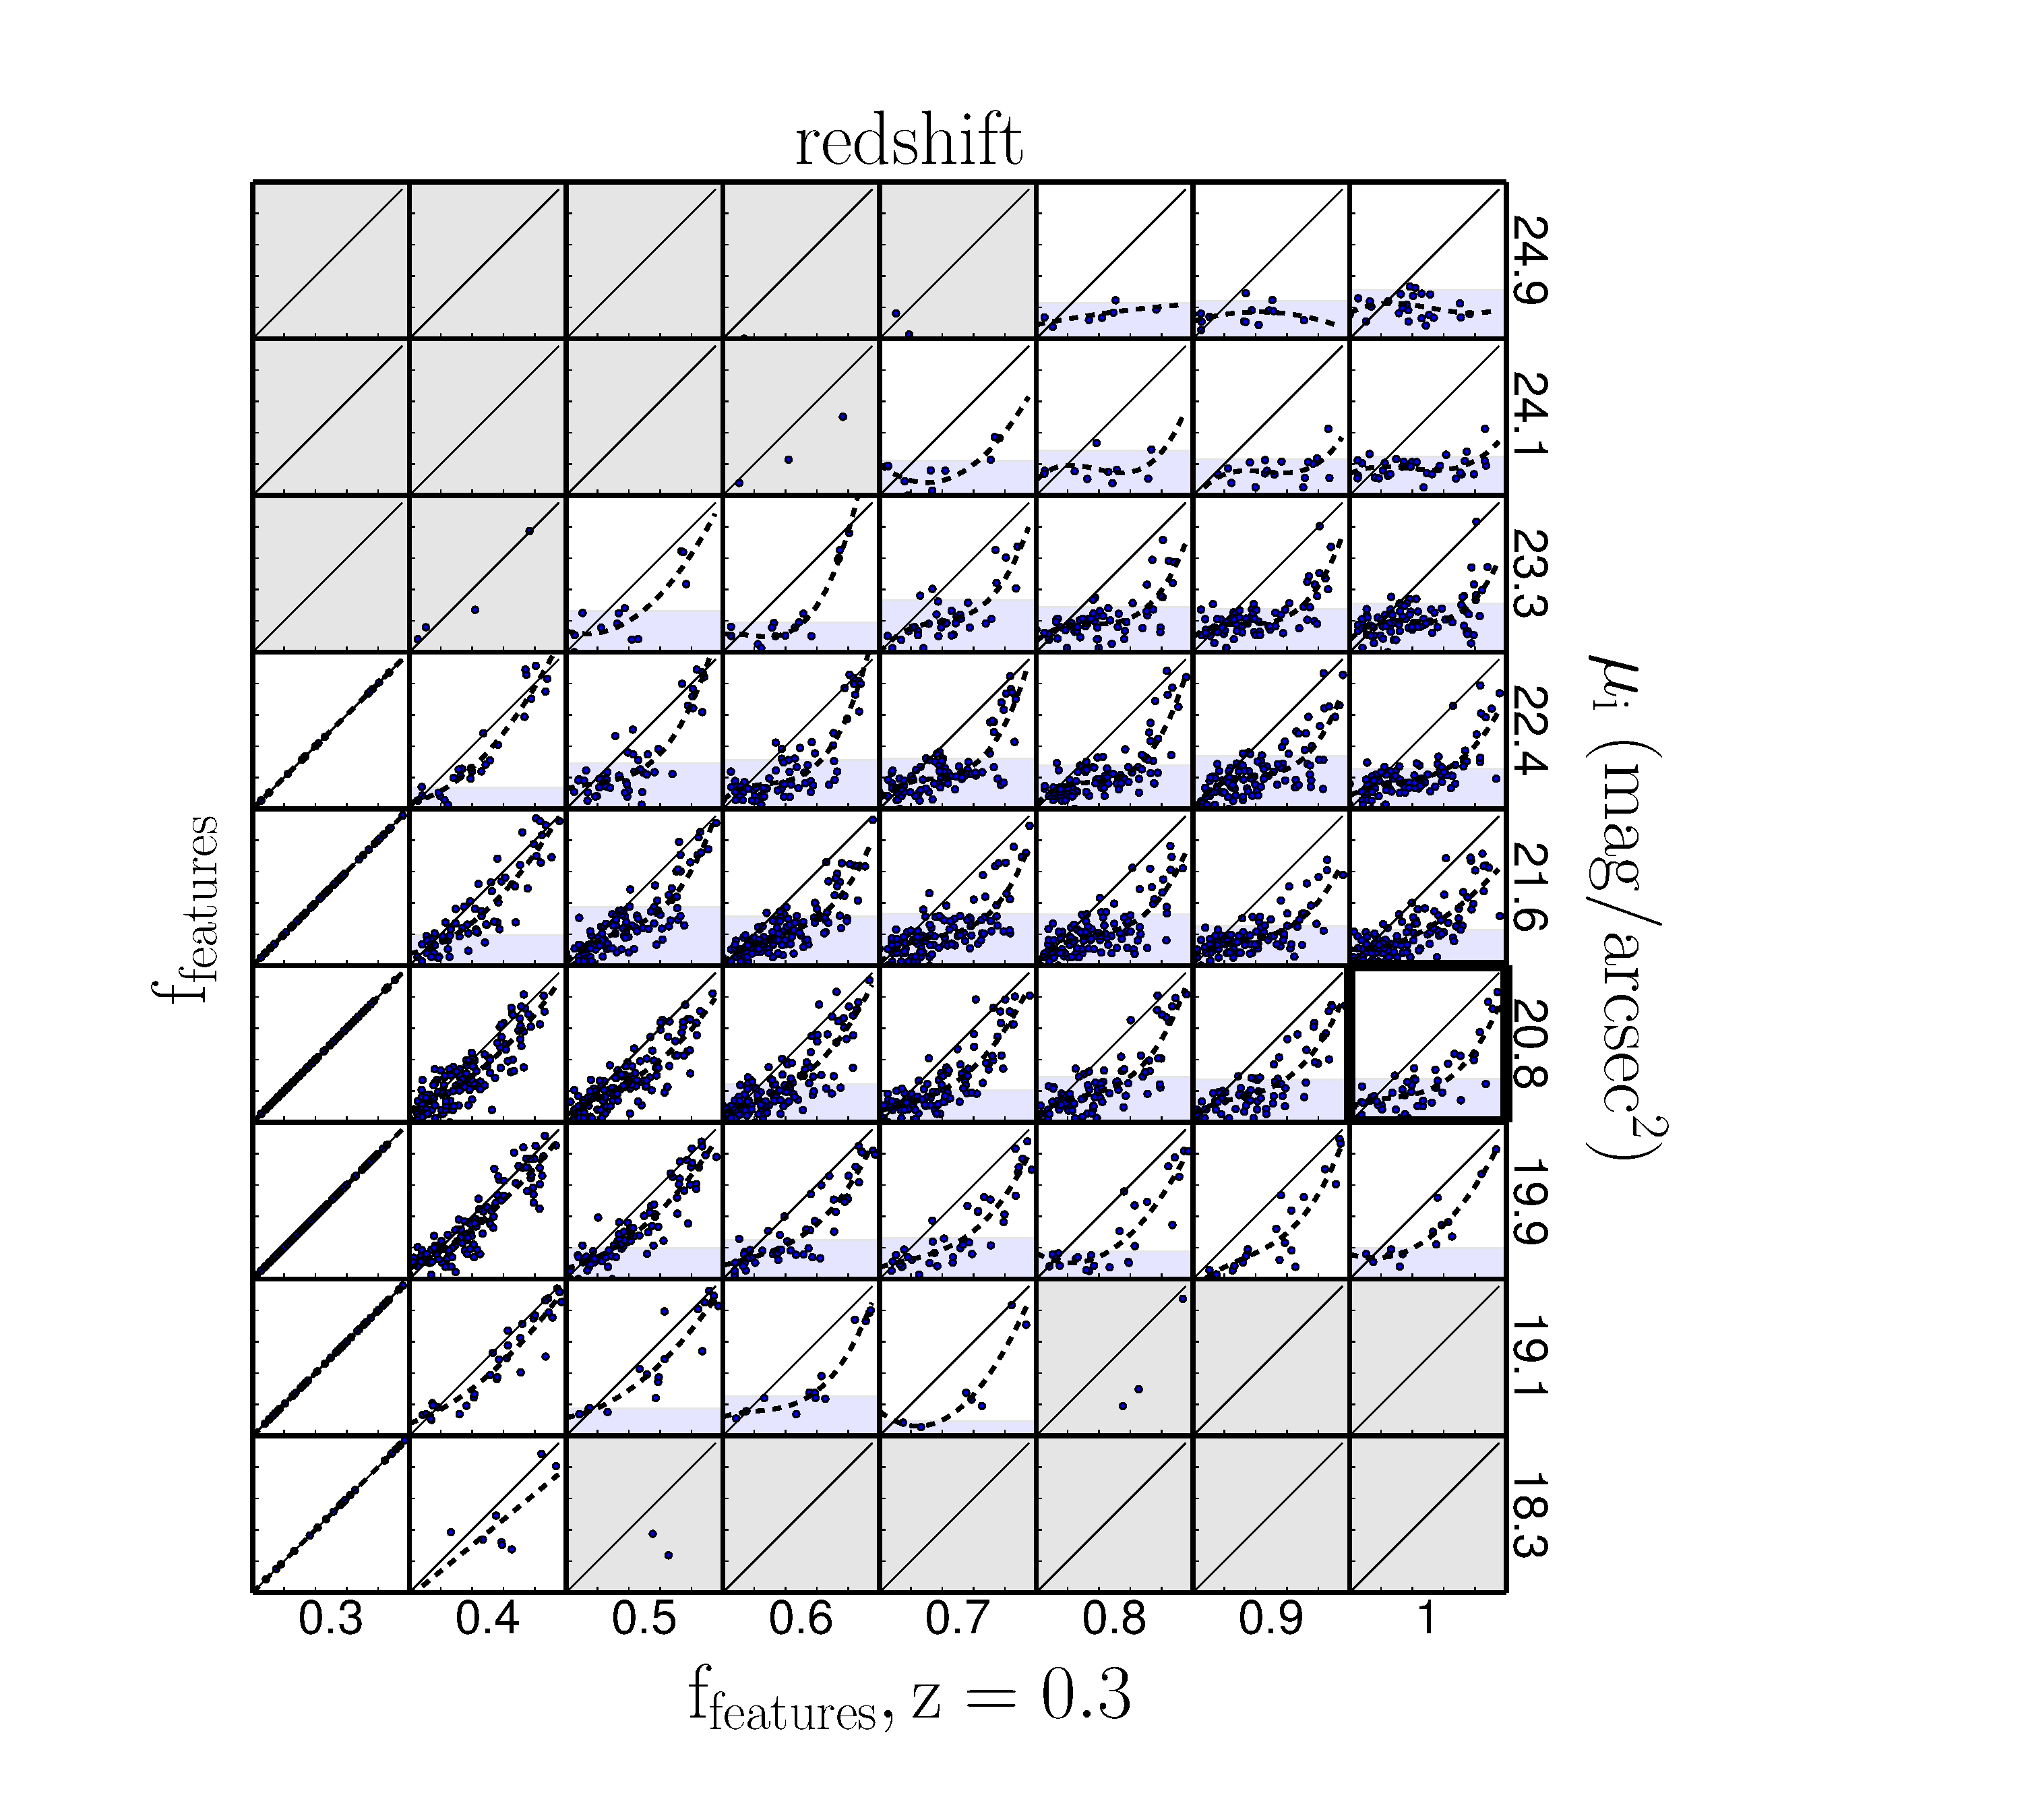
\includegraphics[scale=0.42]{figures/p_vs_p_SB_redshift.pdf}
\caption{Effects of redshift bias in 3,449~images in the \ferengi{} sample.
Each point \emph{in a given redshift and surface brightness bin} represents a
unique galaxy. On the $y$-axis in each bin is the \ffeatures{} value of the
image of that galaxy redshifted to the value corresponding to that redshift
bin. On the $x$-axis is the \ffeatures{} value of the image of the same galaxy
redshifted to $z=0.3$. The dashed black lines represent the best-fit
polynomials to the data in each square. The solid black line represents
\ffeaturesz=\ffeaturesrest. Regions in which there is a single-valued
relationship between \ffeatures{} at high redshift and at $z=0.3$ are white;
those in which there is not are blue, and those with not enough data ($N<5$)
are grey. A larger version of the bin outlined at $z=1.0$ and $20.3 < \mu <
21.0$ $\rm (mag/arcsec^2)$ is shown in Figure~\ref{fig:f_vs_f_zoom}.}
\label{fig:f_vs_f}
\end{center}
\end{figure}

% Figure - small ass plot
\begin{figure}
\centering
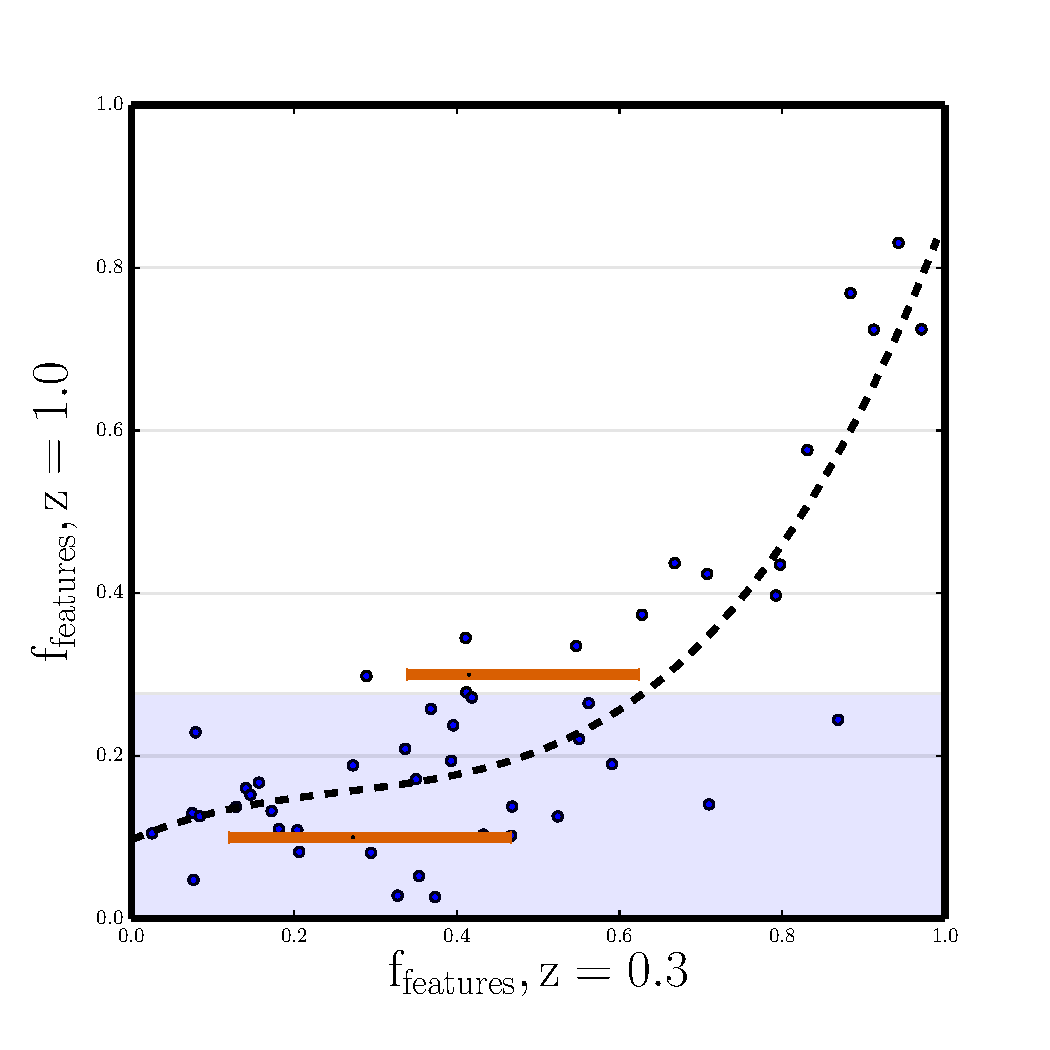
\includegraphics[width=0.7\textwidth]{figures/z1_mu20_subplot2.pdf}
\caption{A larger version of the dark-outlined square in Figure~\ref{fig:f_vs_f}, containing
\ferengi{} galaxies that have been artificially redshifted to $z=1.0$ and have
surface brightnesses between $20.3 < \mu < 21.0$ $\rm (mag/arcsec^2)$. The orange bars represent the inner
68\% (1$\sigma$) of the uncorrectable \ffeatures{} quantiles, which are used
to compute the limits on the range of debiased values.}
\label{fig:f_vs_f_zoom}
\end{figure}

A reliable predicted value can be obtained so long as
the relationship between \ffeaturesz{} and \ffeaturesrest{} is single-valued;
that is, for a given \ffeaturesz, there is exactly one corresponding value of
\ffeatures{} at $z=0.3$. Unfortunately, this is \emph{not} always the case. Figure~\ref{fig:f_vs_f_zoom} shows \ffeatures{} measured at $z=1$ vs \ffeatures{} measured at $z=0.3$ for \ferengi{} galaxies with average surface brightnesses $<\mu>=20.8$ (a zoomed-in version of the dark outlined bin in Figure~\ref{fig:f_vs_f}). This figure shows that if the value of \ffeatures{} measured for a galaxy at $z=1$ is particularly low, there is a wide range that \ffeatures{} could have been if measured at $z=0.3$. Therefore, a low measured value of \ffeatures{} at high redshift could represent two morphological types of galaxies: 1) The galaxy has no distinguishable features and may be classified as a smooth elliptical, or 2) the galaxy \emph{does} have features, but these have become blurred and too difficult to detect at high redshift. 

It is important to identify such regions of surface brightness/redshift/\ffeatures{} space since vote fractions cannot be confidentely corrected to a single value for galaxies in these regions. The criteria for determining whether a region of this space is single-valued, and therefore correctable, is as follows: In each surface brightness and redshift bin, the relationship between \ffeaturesz{} and \ffeaturesrest{} is modelled by fitting the data with polynomials of degress n=3,2, and 1, and using the best formal fit out of the three as measured by the sum of the residuals. These fits are shown as the dashed black lines in Figures~\ref{fig:f_vs_f} and~\ref{fig:f_vs_f_zoom}. Flat regions of the bins are areas in which there is \emph{not} a clear single-valued relationship between \ffeaturesz{} and \ffeaturesrest{}. This is quantified by measuring the slope of the best-fit polynomial to the vote fractions; regions of the bins with a slope less than 0.4 are considered \emph{not} one-to-one, and therefore \ffeaturesz{} cannot be boosted to its \ffeaturesrest{} value. These are colored blue in Figure~\ref{fig:f_vs_f} and are referred to as the \textit{lower limit} sample, because the most stringent correction available is that the weighted \ffeatures{} is a lower limit to the true value.

Correctable and lower-limit regions of $z-\mu$ space can only be identified in bins where there exists a sufficient number of \ferengi{} galaxies to model a polynomial. Bins with fewer than 5 points were not considered sufficiently populated to derive a relationship, and are represented by the gray shaded bins in Figure~\ref{fig:f_vs_f}. Galaxies in the GZH sample whose $z,\mu$ did not correspond to unshaded regions shown in the Figure were assigned to the ``not enough information,'' or ``NEI'' sample, because there were not enough \ferengi{} galaxies to quantify the bias in \ffeatures{} in that parameter space. Figure~\ref{fig:eye_of_sauron} displays the overlap of $z,\mu$ bivariate distributions of the GZH and \ferengi{} samples. Ideally, the \ferengi{} space would overlap the GZH parameter space as close as possible. However, the unfortunate consequence of the simulated set being derived from galaxies in the local Universe puts an upper limit on the maximum surface brightness achievable for the \ferengi{} set. The earlier Universe simply has many more galaxies at the high surface brightness end, which were reproduced as best as possible by applying the magnitude correction, but ultimately can only result in a distribution that spans, but not completely reproduces, the bivariate distribution of the real data. The mismatch should not affect the overall calibration accuracy of the debiasing method, since only galaxies in particular $z-\mu$ bins are being corrected. It was stressed in the data release \citep{Willett2016} however that due to this limitation in parameter space, all corrected values should be used with caution when using them for population studies.  

%Figure: compare z/mu distribution of hubble and ferengi sample
\begin{figure}
\begin{center}
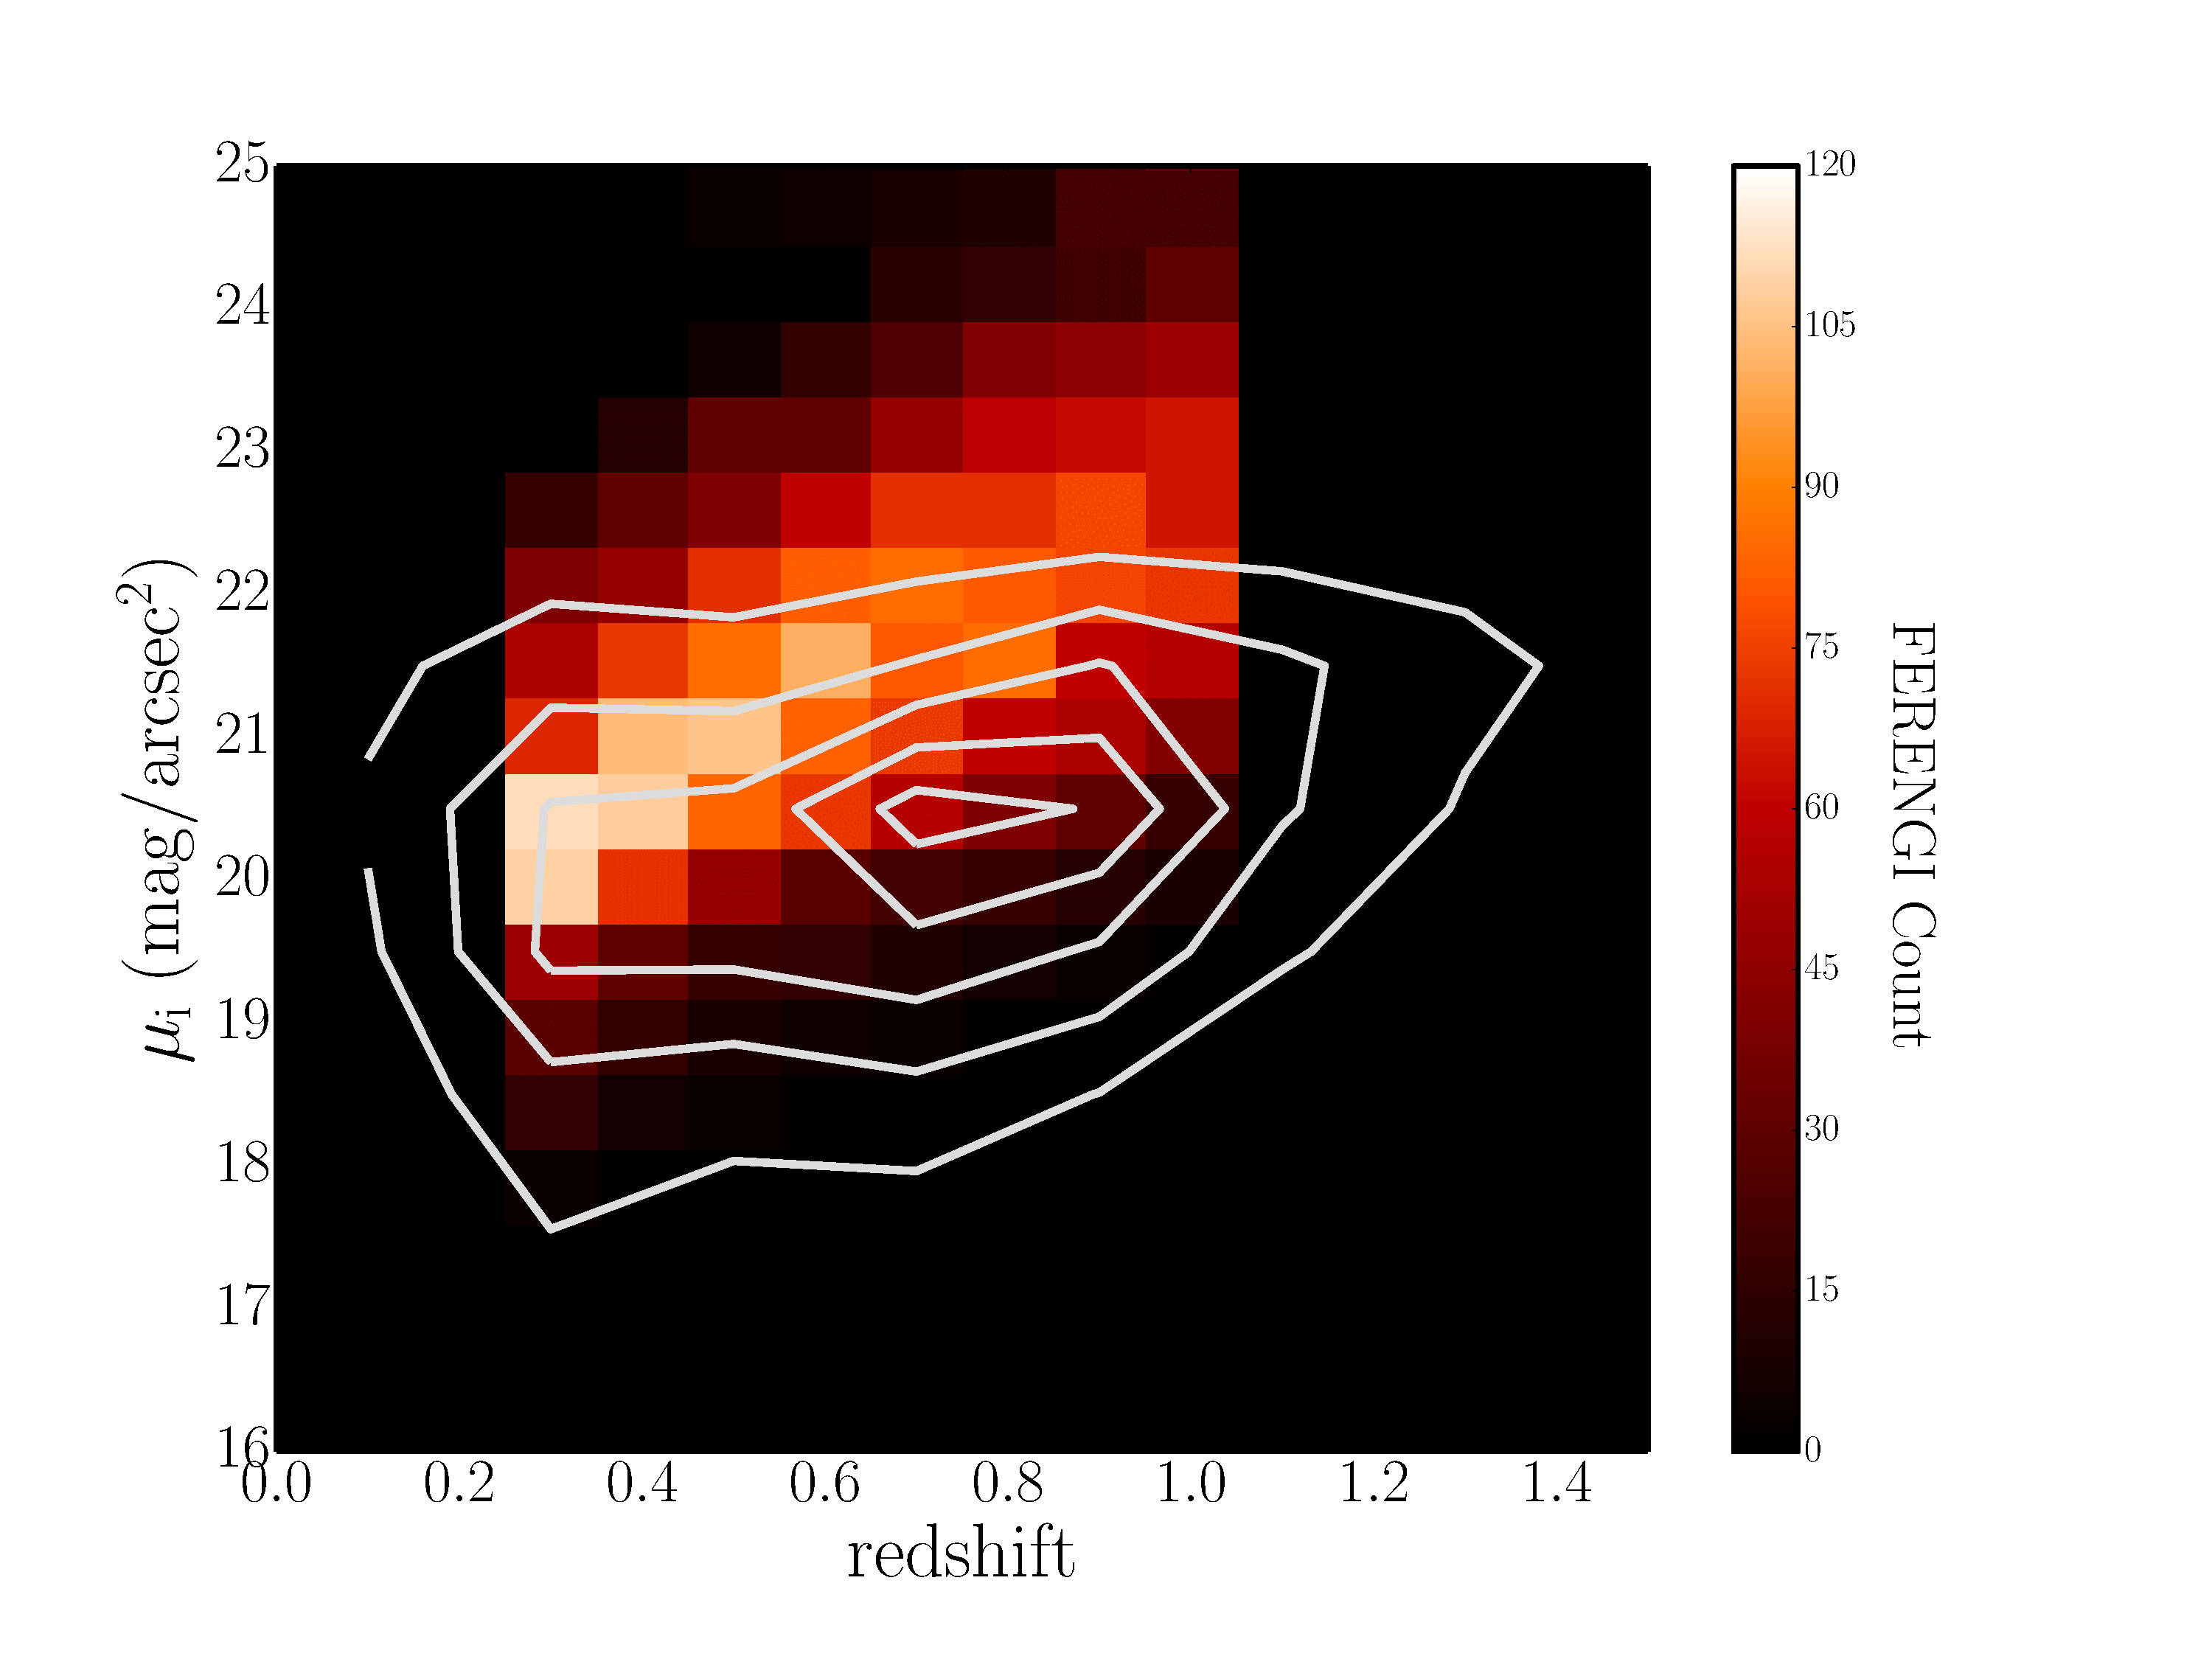
\includegraphics[width=0.6\textwidth]{figures/eye_of_sauron.pdf}
\caption{Surface brightness as a function of redshift for 3,449~\ferengi{}
images and the 102,548~\main{} galaxies with measured $\mu$ and $z$ values. The
colour histogram shows the number of \ferengi{} images as a function of $\mu$
and $z_{\rm sim}$. White contours show counts for the galaxies in the \main{}
sample, with the outermost contour starting at $N=1500$ and separated by
intervals of 1500.} 
\label{fig:eye_of_sauron}
\end{center}
\end{figure}


The unshaded regions of Figure\ref{fig:f_vs_f_zoom} thus define descrete ranges of redshift, surface brightness, and \ffeatures{} within which a galaxy must lie in order for the debiased vote fraction to be confidentely applied. While the appropriate correctable regions were defined as discrete bins, the true correctable region is assumed to be a smooth function of $z, \mu,$ and \ffeatures{}. To define this smooth space, a convex hull was calculated to enclose the correctable and lower-limit \ferengi{} galaxies in the $z-\mu-$\ffeatures{} space (see Figure~\ref{fig:hull}). The space defined by this hull was used to ultimately separate the GZH galaxies into correctable samples (those for which a correction to \ffeatures{} can confidentely be applied, see next section) and lower-limit samples (those for which a single-valued correction cannot be applied). The final categorization of the GZH sample, split by imaging survey, is shown in Table~\ref{tab:hubble_debiasable}. 
% Figure - convex hull
\begin{figure}
\centering
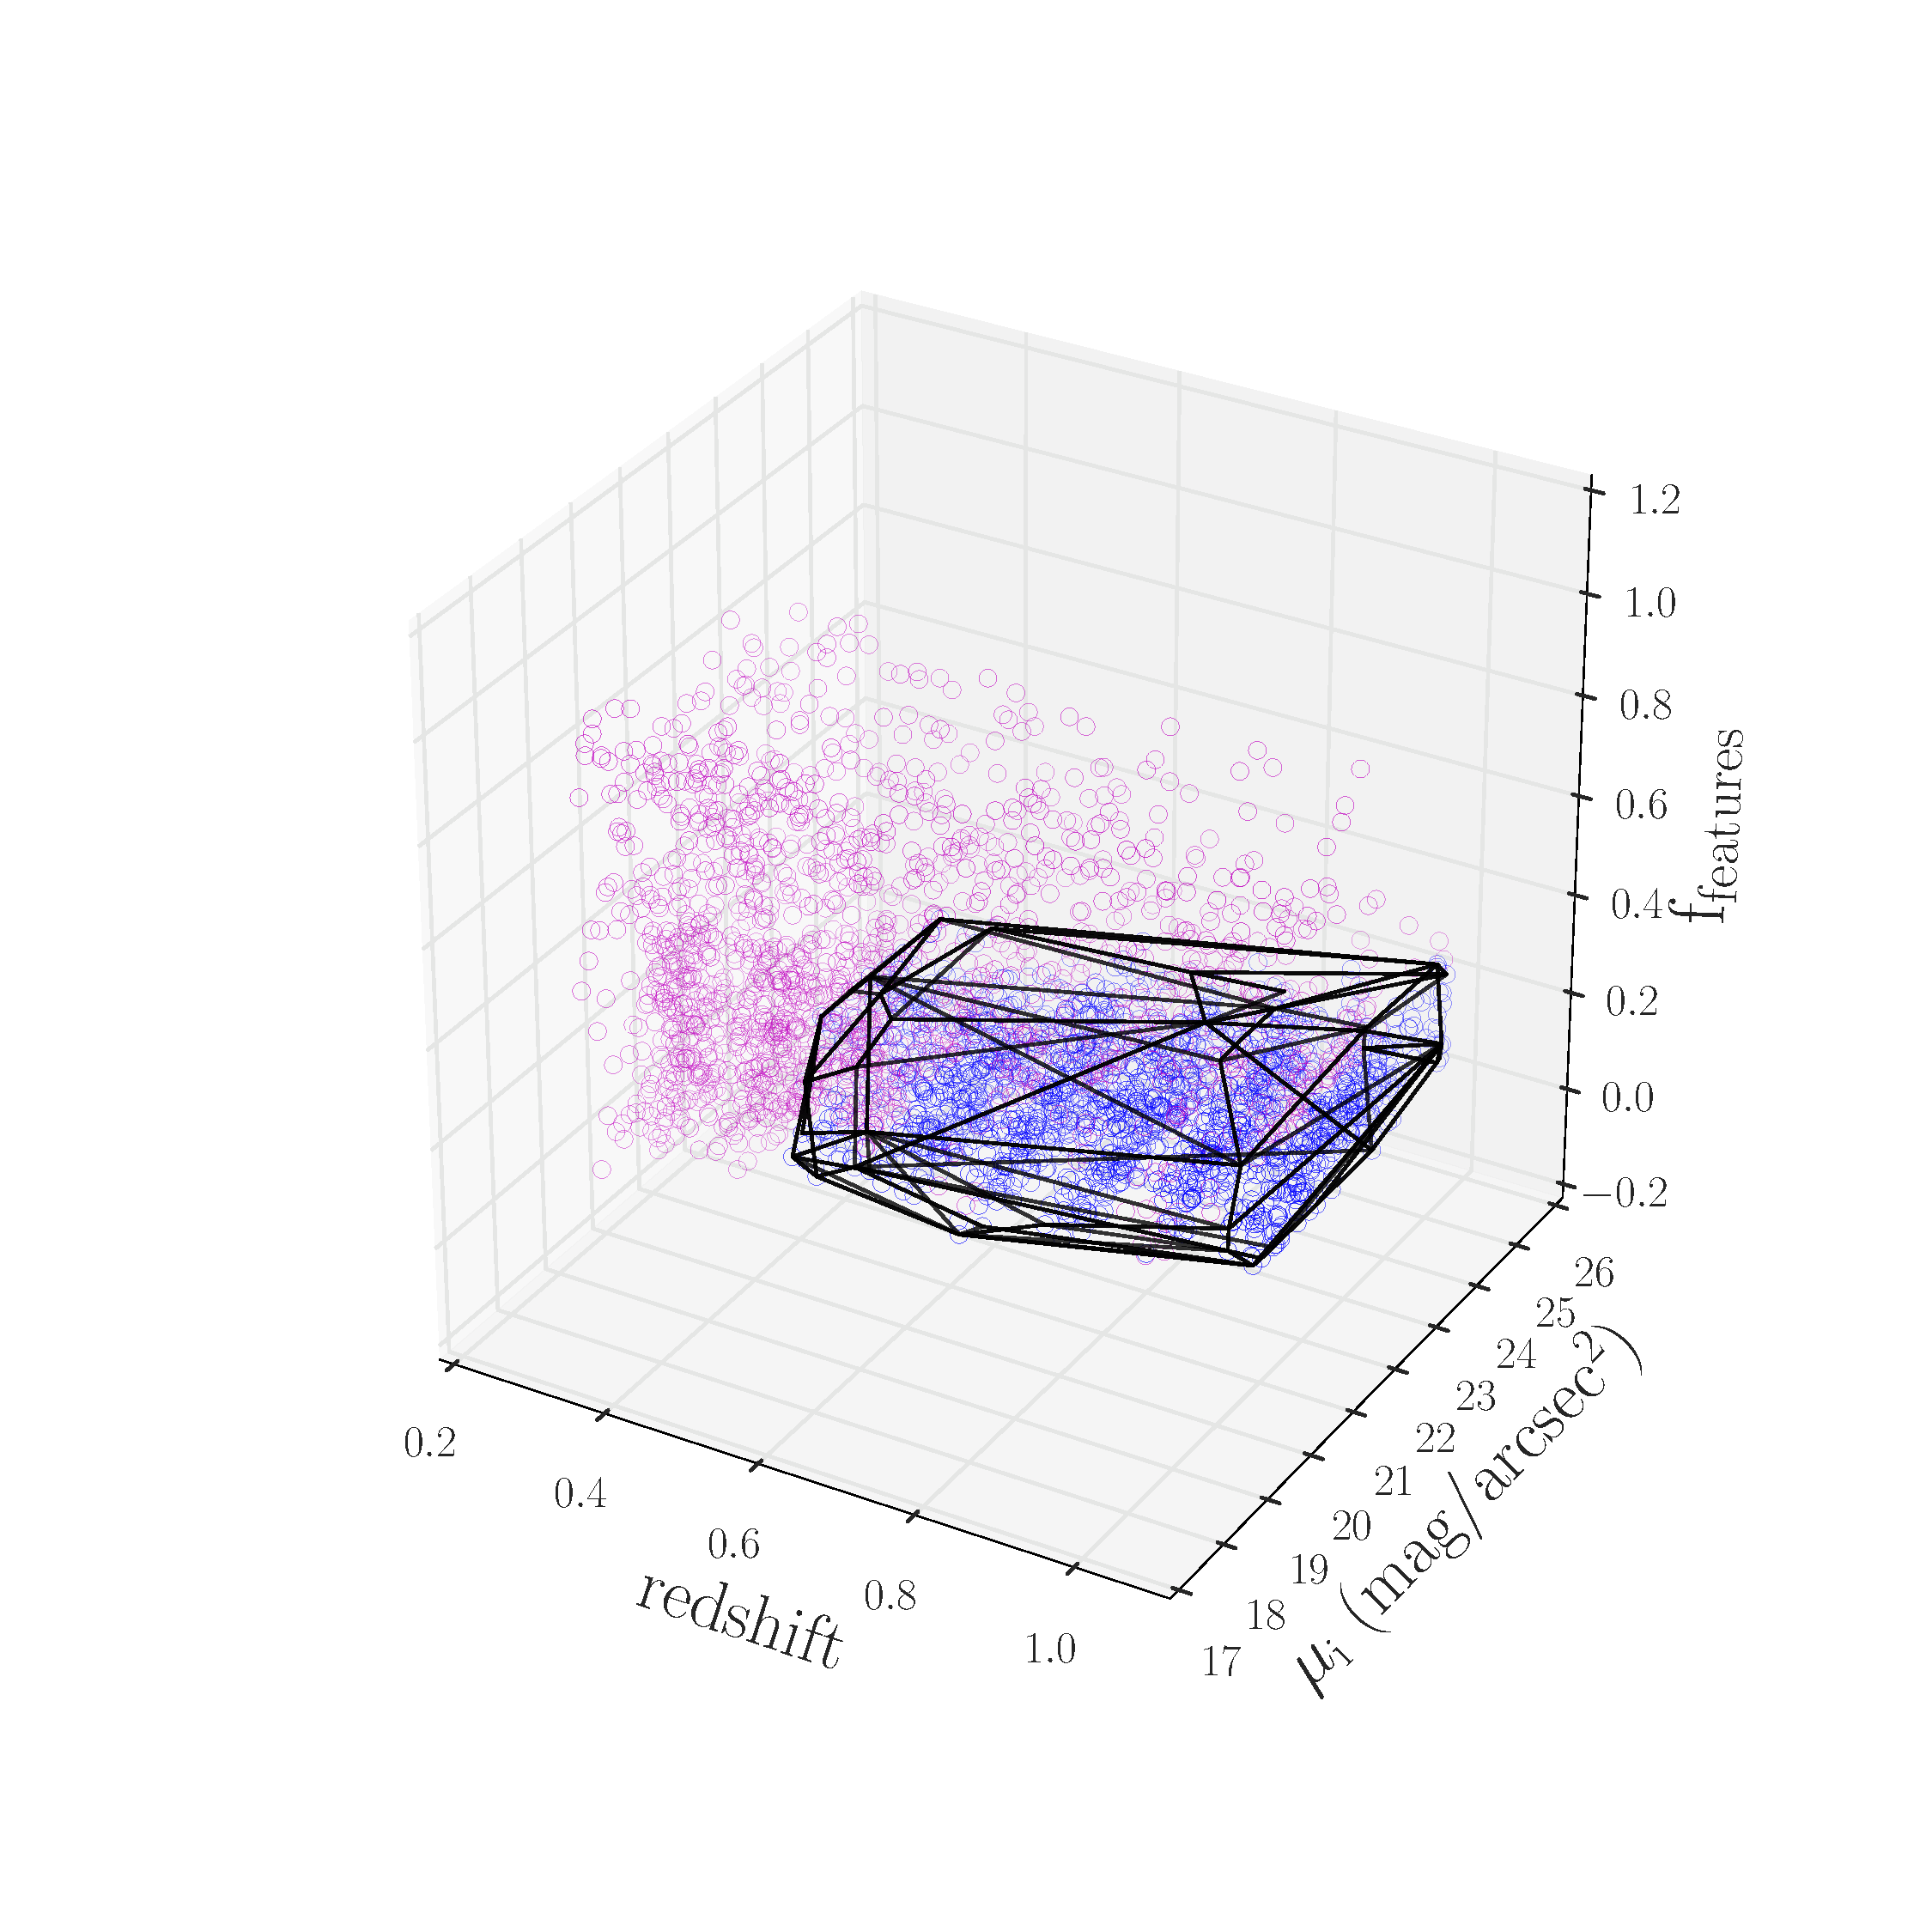
\includegraphics[width=\textwidth]{figures/convex_hull.pdf}
\caption{The final separation of the correctable and lower-limit samples in redshift/surface brightness/\ffeatures{} space.\textbf{Pink} points are all \ferengi{} galaxies in the \textbf{unshaded} regions of Figure~\ref{fig:f_vs_f}. \textbf{Blue} points are all \ferengi{} galaxies in the \textbf{blue shaded} regions of Figure~\ref{fig:f_vs_f}. The solid black line is the convex hull which encloses the uncorrectable points and defines the region of the lower-limit sample. }
\label{fig:hull}
\end{figure}



%Table: distribution of correction types for HST
\begin{table}
\rotate
\caption{Number of correctable galaxies for the top-level task in GZH, split by \hst{} survey.}\label{tab:hubble_debiasable}
\begin{tabular}{lcrrrrr|r}
\hline\hline
                    & Correction type & AEGIS   & COSMOS & GEMS  & GOODS-N & GOODS-S  &  Total  \\
                    &                 &         &        &       & 5-epoch & 5-epoch  &         \\
\hline
correctable         & 0               & 2,908   & 21,169 & 2,802 & 1,459   & 1,189    &  29,527 \\
lower-limit         & 1               &   833   &  5,169 & 1,021 & 1,377   & 1,267    &   9,667 \\
$z \le 0.3$         & 2               &   955   & 10,870 & 1,175 &   415   &   400    &  13,815 \\ 
NEI                 & 3               & 2,677   & 43,058 & 3,559 & 2,077   & 2,184    &  53,555 \\
no $z$ info         & 4               & 1,134   &  4,688 &   530 &   687   &   102    &   7,141 \\
\hline
total               &                 & 8,507   & 84,954 & 9,087 & 6,015   & 5,142    & 113,705 \\
\hline\hline
\end{tabular}
\end{table}


For the ``lower limit'' galaxies, since a single debiased \ffeatures{} value cannot be confidentely assigned, a \emph{range} of debiased values is estimated. In each $z,\mu$ bin in Figure~\ref{fig:f_vs_f}, the spread of intrinsic values of \ffeaturesrest{} for five quantiles of observed \ffeatures{} is computed - these are denoted by the gray lines in the close-up Figure~\ref{fig:f_vs_f_zoom}. The range of intrinsic values of \ffeatures{} is defined by the upper and lower 1 $\sigma$ limits, enclosing the inner 68\% of the data; this is represented by the orange bars in Figure~\ref{fig:f_vs_f_zoom}. For any galaxy which cannot be directly debiased, these ranges are used to denote the upper and lower limits on the expected values \ffeaturesrest{} as a function of the observed \ffeatures{}. 

\subsection{The $\zeta$ equation}

For the ``correctable'' sample of simulated \ferengi{} galaxies, an equation was derived to model the dropoff in \ffeatures{} with redshift for each galaxy. Such a model is assumed to have the following criteria: (1) For a given galaxy, \ffeatures{} should decrease relative to its \ffeaturesrest{} as redshift increases. (2) The corrected \ffeatures{} value must be contained within 0 and 1, since it is a fraction. (3) The degree of dropoff may depend on the surface brightness of the galaxy. Given these three assumptions, a simple exponential function was derived:

\begin{equation}
f_{\mu,z} = 1 - (1 - f_{\mu,z=0.3})e^{\frac{z-z_0}{\hat\zeta}}
\label{eqn:fzeta}
\end{equation}

where $f_{\mu,z=0.3}$ is the vote fraction at the lowest redshift in the artificially-redshifted \ferengi{} sample ($z_{0}=0.3$). $\zeta$ is a parameter that controls the rate at which \ffeatures{} decreases with redshift. 

\begin{figure*}
\center
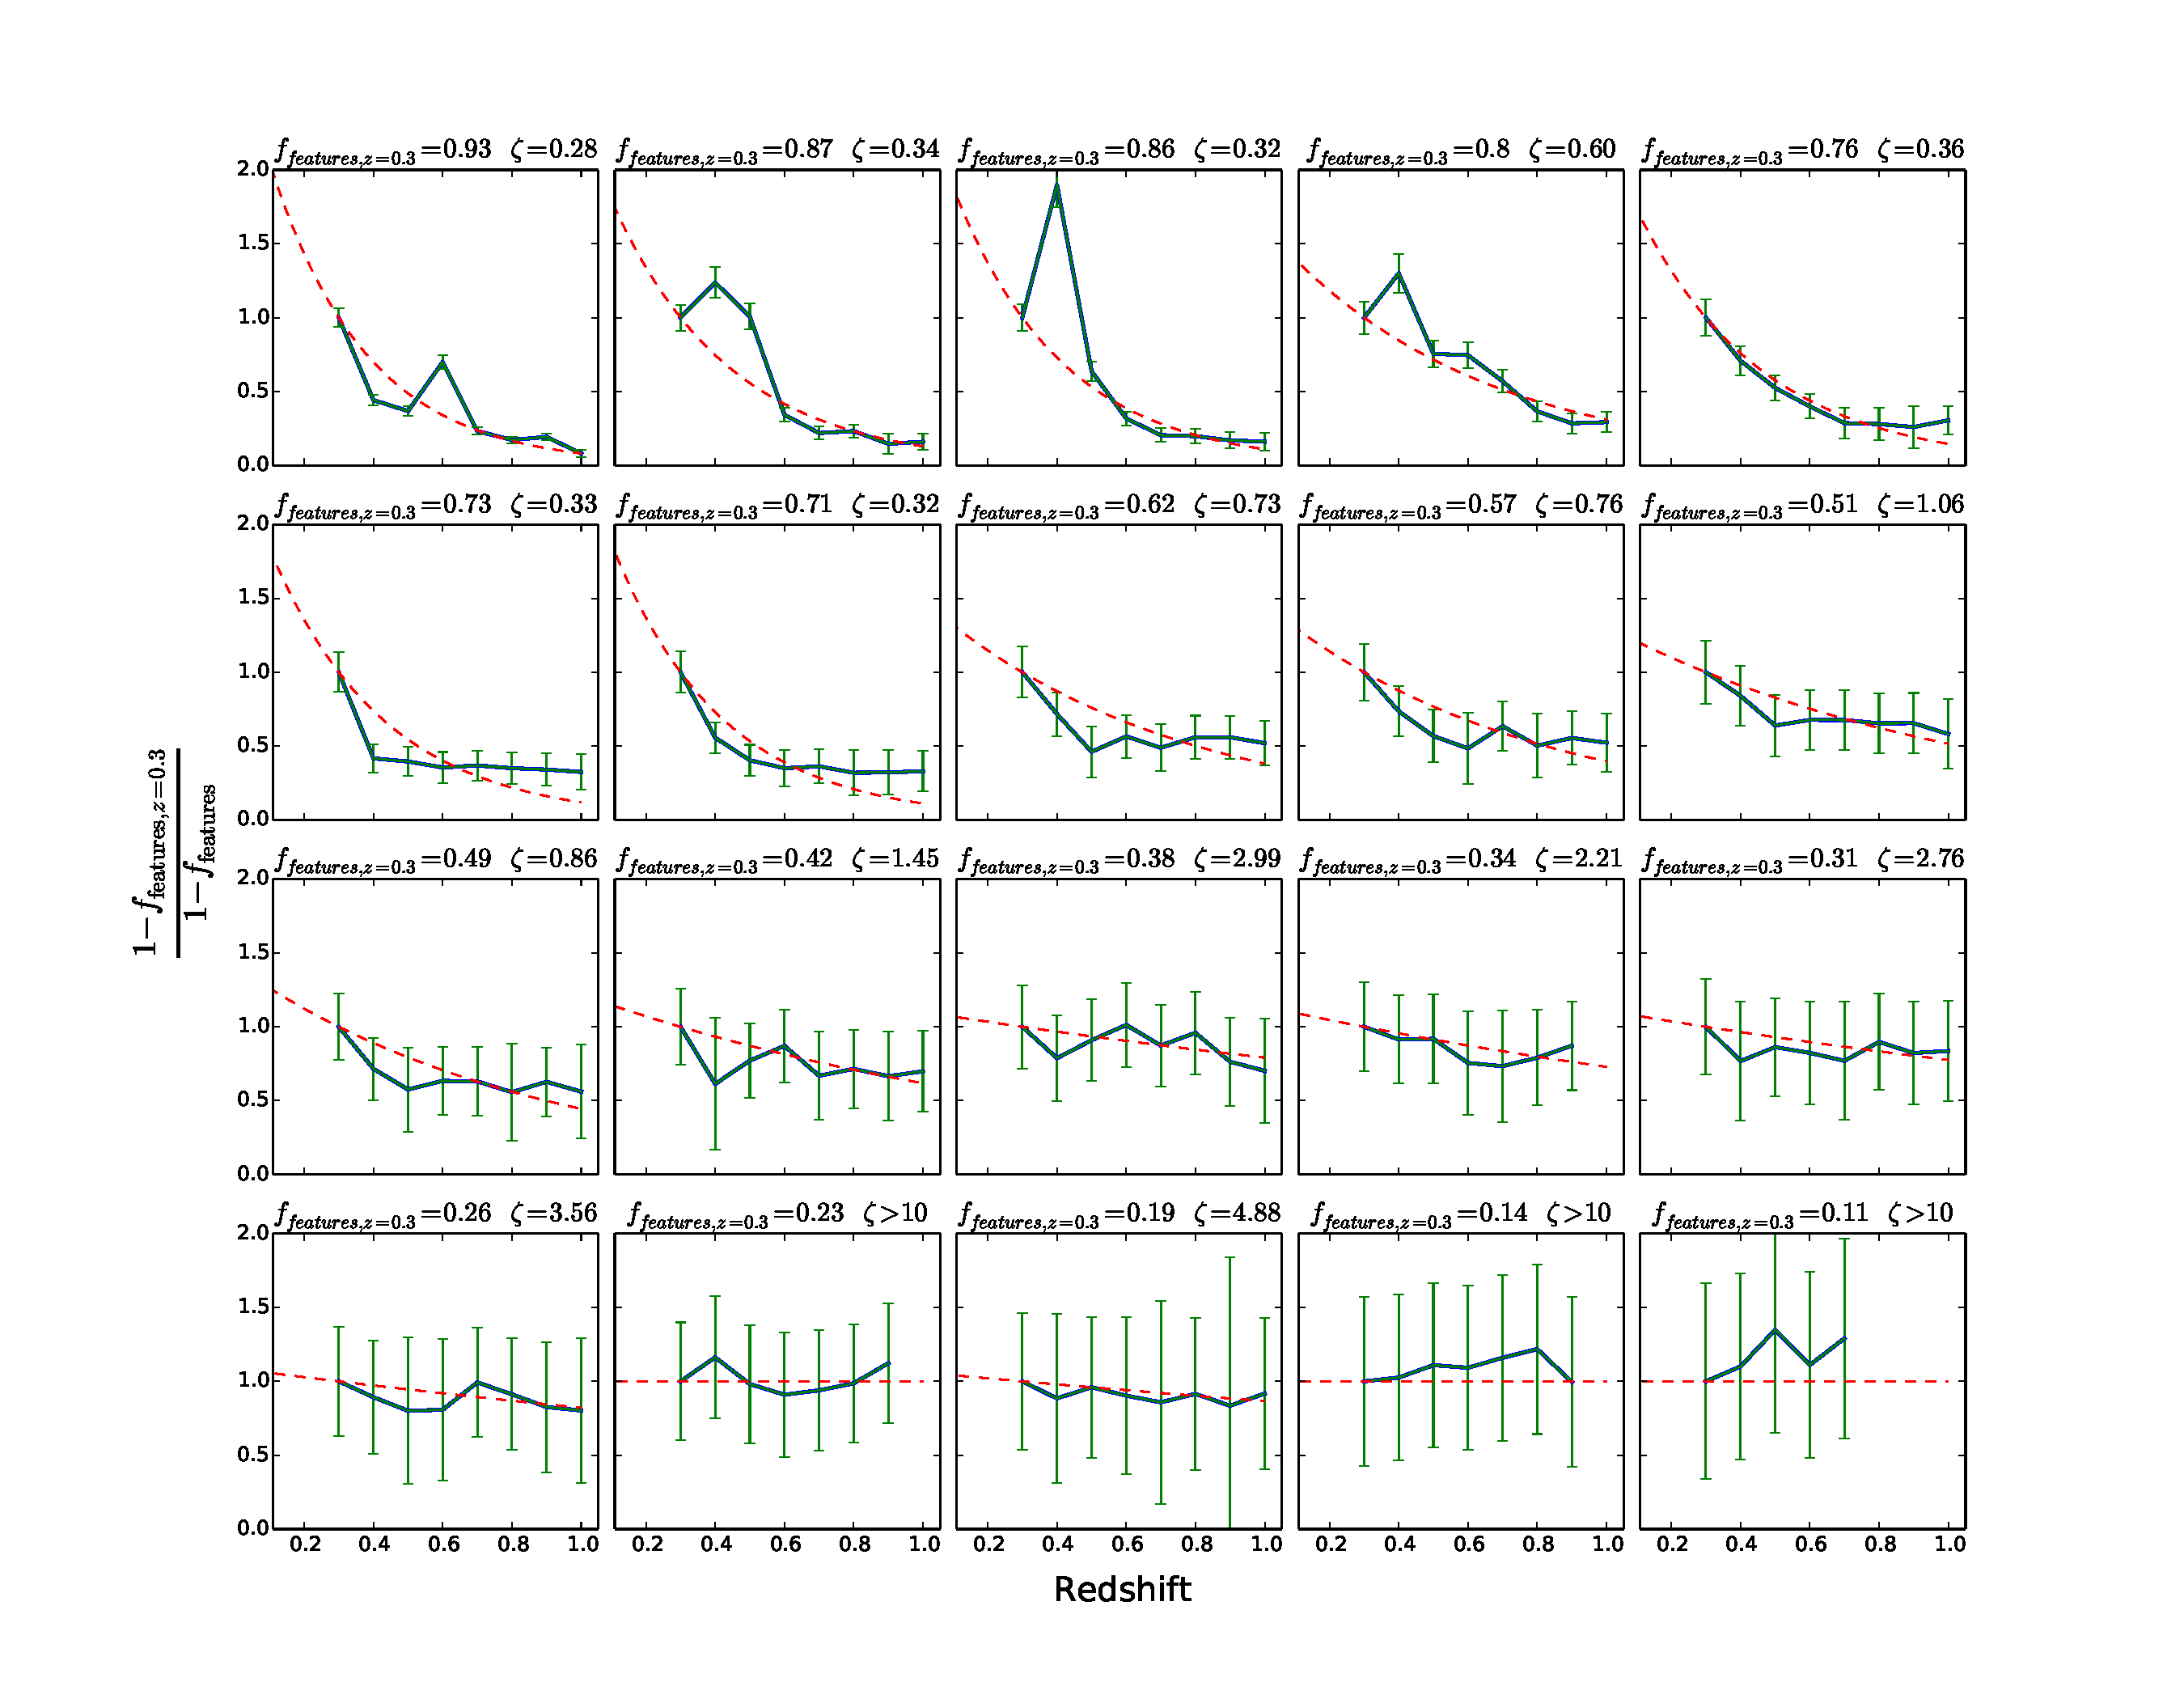
\includegraphics[width=\textwidth]{figures/zeta_examples_sorted.pdf}
\caption{Behavior of the normalised, weighted vote fractions of features
visible in a galaxy ($f_\textrm{features}$) as a function of redshift in the
artificial \ferengi{} images. Galaxies in this plot were randomly selected from
a distribution with evolutionary correction $e=0$ and at least three detectable images 
in redshift bins of $z\ge0.3$. The displayed bins are sorted by \ffeaturesrest, 
labeled above each plot. Measured vote fractions (blue
solid line) are fit with an exponential function (red dashed line;
Equation~\ref{eqn:fzeta}); the best-fit parameter for $\zeta$ is given above
each plot.}


% Error bars are binomial for each f, symmetrised, then added in quadrature.
\label{fig:zeta_examples}
\end{figure*}



Equation~\ref{eqn:fzeta} was then fit to each galaxy in the ``correctable'' \ferengi{} sample, and $\zeta$ is measured for each. Figure~\ref{fig:zeta_examples} shows the best fit equations for 16 galaxies, and the $\zeta$ corresponding to the best fit is displayed with each galaxy. As it was assumed that surface brightness likely plays a role in the level of dropoff in \ffeatures{}, and hence the value of $\zeta$ which controls this dropoff, it is assumed that $\zeta$ follows a simple linear dependence with surface brightness:


\begin{equation}
\log_{10}(\hat\zeta) = \zeta_0 + (\zeta_1 \times \mu),
\label{eqn:zetafit}
\end{equation}

where $\hat\zeta$ is the correction factor applied to each galaxy. Figure~\ref{fig:zeta_mu} shows the relationship between the derived $\zeta$ values and the surface brightness $\mu$ of the \ferengi{} galaxies, which is fit with equation~\ref{eqn:zetafit}. The best-fit parameters to this linear fit from least-squares optimization are  $\zeta_0=0.50$, $\zeta_1=-0.03$. Interestingly, only a very weak surface brightness dependence is detected. It is difficult to determine from these data whether the weak detection is due to a true lack of dependence, or insufficient data (only 28 galaxies had sufficient data to accurately measure $\zeta$). 

\begin{figure}
\center
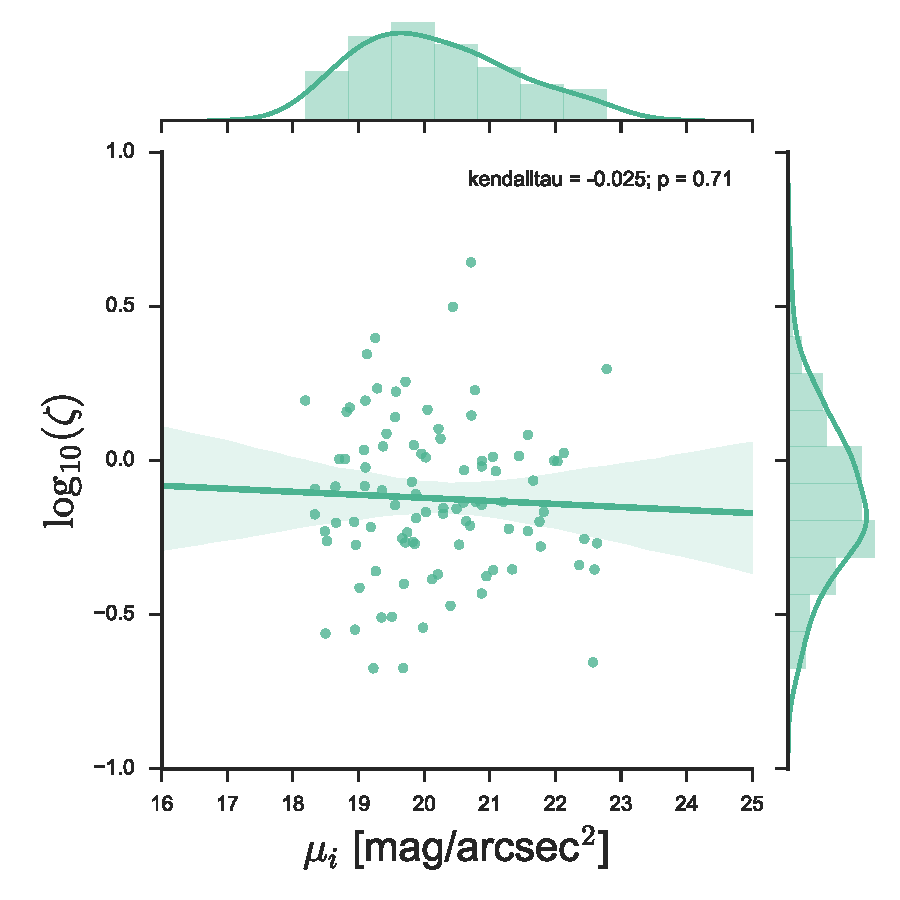
\includegraphics[width=0.6\textwidth]{figures/zeta_mu.pdf}
\caption{All fits for the \ferengi{} galaxies of the vote fraction dropoff
parameter $\zeta$ for \ffeatures{} as a function of surface brightness. This
includes only the simulated galaxies with a bounded range on the dropoff
($-10<\zeta<10$) and sufficient points to fit each function (28~original
galaxies, each with varying images artificially redshifted in one to eight bins over a range from $0.3\lesssim z_\mathrm{sim}\lesssim1.0$).}

\label{fig:zeta_mu}
\end{figure}


Using the $\zeta$ parameters measured in the \ferengi{} sample, a final debiased correction equation is derived to correct the \ffeatures{} vote fractions in the HST data:
\begin{equation}
f_\textrm{features,debiased} = 1 - (1 - f_\mathrm{features,weighted})e^{\frac{-(z-z_0)}{\hat\zeta}}
\label{eqn:fzeta_mod}
\end{equation}

\noindent where $f_\mathrm{features,weighted}$ is the weighted vote fraction, and $f_{\rm features,debiased}$ is bounded 
between $f_{\rm features,weighted}$ and 1. 

%Figure: showing correctable sample in  redshift/ffeatures space 
\begin{figure}
\center
\includegraphics[width=\textwidth,trim={0cm 2cm 0cm 1cm},clip]{figures/correctable_space.pdf}
\caption{\textbf{Left}: Debiased vs raw vote fractions for the GZH correctable sample. \textbf{Right}: Histogram showing the fraction of galaxies that have a finite correction for the debiased vote fractions \ffeaturesdebiased{} as a function of \ffeatures{}
and redshift. The parameter space for corrections is limited to $0.3 \leq z \leq 1.0$
due to the sampling of the parent SDSS galaxies and detectability in the \ferengi{} images.
}
\label{fig:correctable_fraction}
\end{figure}



\subsection{Debiasing results and limitations of the \ferengi{} simulated data}
Figure~\ref{fig:correctable_fraction} shows the results of the $\zeta$ correction for the correctable sample. Plotted on the left panel is the corrected ($\hat f_{features}$) vs the raw (\ffeatures{}) fractions. Galaxies with low ($ f_{features} < 0.2$) may be corrected to as high as $\sim 0.6$, while fractions already large require no additional boost. Using the corrected values will aid in the identification of featured galaxies in future studies. The limitations of the process can be seen in the right panel of the figure. Displayed is the fraction of galaxies in the correctable sample as a function of redshift and initial \ffeatures{}. At the low end of \ffeatures{}, only galaxies also with low redshifts tend to be a part of the sample; this is due to the effect desribed above wherein the low resolution of the high-redshift images reaching a point where smooth-appearing featured galaxies are completely indiscernable from ellipticals, and it is not possible to be certain that a boost is necessary. This limitation is unavoidable given the limited sensitivity of any instrument, however this effect will be lessened as imaging technology continues to improve. 

The \ferengi{} sample was successful in identifying and correcting the vote fractions of the GZH sample to aid in identifying featured galaxies, albeit with several limitations. Inspired by the utility of the simulated galaxy classifications, a second set was created for a very specific purpose of measuring the incompleteness in disk \emph{fraction} (as opposed to incompleteness in individual vote fractions). The second half of this Chapter will explain the motivations behind and the generation of this second simulated set.
 
\section{Ferengi 2: using simulated images to measure incompleteness in disk fraction}

In the previous section I described how we used the simulted \ferengi{} images to measure the redshift/surface brightness dependence on \ffeatures, and applied the measurements towards a correction factor to the vote fractions directly. In this section I will describe the motivation, selection, and application of a second set of \ferengi{} images used to measure and correct for the incompleteness in \emph{number} of disks detected as a function of redshift and surface brightness, used in the work described in Chapter~\ref{chap:gzh_red_disks}.

\subsection{The Ferengi 2 Sample}
\label{ssec:ferengi2sample}

The creation of a second set of \ferengi{} images was motivated by the scientific goal of measuring the redshift evolution of the fraction of red disk galaxies using the Galaxy Zoo: Hubble dataset. This project is described in full in Chapter~\ref{chap:gzh_red_disks}, but the reasons requiring a new set of simulated images will be described briefly here. First, as described in the previous section, the analysis of the first \ferengi{} set revealed that, for a large area of z-$\mu$ parameter space, galaxies with low measured values of \ffeatures{} could not be corrected to a point that could clearly distingush them as disks with washed-out features or ellipticals. Due to this limitation, any measurement of the number of disk galaxies in a given redshift interval can only be reported as a \emph{lower-limit} to the true value. The difference in the measured lower-limit and the true number of disks is what we will refer to as the \emph{incompleteness} in number of disks detected. 

It is possible, then, to use the \ferengi{} images to measure this incompleteness by measuring the number of disks detected at a given redshift, and comparing to the number of disks detected out of the same galaxies at the lowest redshift (this would be considred the true, or intrinsic, number of disks.) The details of this approach will be described in the next section. A complication specific to this project is that the number of disks will be ultimitely used to compute the \emph{red disk fraction}, that is, the ratio of the number of red disks to all disks, as a function of redshift. It is then necessary to measure the level of incompleteness for both red and blue galaxies separately, to calculate this fraction most accurately.

The color separation method for the \hst~galaxies in Chapter~\ref{chap:gzh_red_disks} uses NUV, r, and J magnitudes. To separate the \ferengi{} sample of galaxies into red and blue samples in the same way, these magnitudes are required. In the first set, however, only 44 of the 288 galaxies had these data available, which were not enough to properly measure any incompleteness, especially after binning the data further in surface brightness and redshift. So, a larger set of galaxies to be artificially redshifted, all which had the aforementioned data necessary to separate by color, was required.

This set of new galaxies to be put through the \ferengi{} code, hereafter refered to as the \ferengi{} 2 sample, was selected as follows: All candidates were pulled from a parent sample of all SDSS galaxies which had previously been classified in GZ2. As discussed in Section~\ref{sec:ferengi1sample}, only galaxies with redshifts below $z<0.013$ were able to be redshifted the full simulated redshift range $0.3<z<1.0$, so a redshift cut was implemented of $z<0.013$. These galaxies were cross-matched with catalogs from GALEX \citep{Martin2005} for NUV magnitudes and 2MASS \citep{Skrutskie2006} for J magnitudes. 1,435 galaxies fit these criteria.  

Bulk SDSS u, g, r, i, and z-band fits images were then downloaded for all 1,435 galaxy candidates \footnote{http://data.sdss3.org/bulkFields}. Cutouts were made for each galaxy, using the 90\% r-band petrosian radius to set the size of the cutout (\radr). The default prescription used was to define the edges as 2.5*\radr, measured from the galaxy as the center. If the galaxy was within this distance from the edge of the bulk fits image, 2.0*\radr~was used. Cutouts were not made for galaxies within this distance from the edge, both to ensure the full galaxy was visible in all cutouts in the sample, and to avoid over-zooming the image. 187 galaxies were thus removed from \ferengi 2; an example of such a galaxy ``too close'' to the edge of the edge is shown in Figure~\ref{fig:edge_galaxy}.  



%Figure: galaxy cutouts
\begin{figure}
\begin{center}
\includegraphics[width=0.9\textwidth]{figures/edge_galaxy.png}
\caption{Example of a galaxy overlapping the edge of the SDSS frame. Shown is the bulk r-band fits image for SDSS DR12 run 3903, camcol 6, and field 60. The boxed-in galaxy (SDSS DR12 objid 1237662239079268544) is too close to the edge of the image to create a cutout that encloses the entire galaxy. The pink dashed box indicates a cutout size of 2*\radr, the blue solid line indicates a cutout size of 2.5*\radr. } 
\label{fig:edge_galaxy}
\end{center}
\end{figure}

While all 78 $z<0.013$ galaxies from the original \ferengi{} sample were successfuly simulated to a minimum redshift of $z_{sim}=0.3$, this was not always true for the \ferengi 2 candidates. Redshift of the source galaxy is the largest factor in determining the minimum possible simulated redshift, but other factors including the size of the psf and physical size of the source galaxy also come into play. All 1,248 candidates were then put through \ferengi{} at only the lowest redshift $z_{sim}=0.3$ to begin, and each image was visualy inspected to determine whether the code succeeded. 312 ``failures'' were detected; two examples are shown in Figure~\ref{fig:ferengi_fails}. The remaining 936 ``successes'' were then artificially redshift the full range of $0.3<z<1.0$ in increments of $dz = 0.1$; these make up the final \ferengi 2 sample of 7,488 images of 936 galaxies redshifted 8 times. A single evolution factor, rather than a range, of $e=1$ was applied to all images. This value was chosen by analyzing the spectra template models of \cite{Brinchmann2004a}, which showed that the most typical galaxies evolve in brightness by one magnitude per redshift. Example images are shown in Figure~\ref{fig:ferengi2_examples}


%Figure: ferengi2 fails
\begin{figure}
\begin{center}
\includegraphics[width=\textwidth]{figures/failed_ferengis.png}
\caption{Examples of two galaxies whose minimum simulated redshifts in \ferengi{} were larger than $z_{sim}=0.3$. These were detected via visual inspection and removed from the final \ferengi 2 sample.} 
\label{fig:ferengi_fails}
\end{center}
\end{figure}


%Figure: ferengi2 examples
\begin{figure}
\centering
\includegraphics[width=\textwidth]{figures/ferengi2_examples.png}
\caption{Examples of \ferengi 2 galaxies. The left is the original gri-composite image of the source galaxy. Images on the right are simulated output from the \ferengi{} code. Only four of the eight simulated redshifts are shown in the interest of space.} 
\label{fig:ferengi2_examples}
\end{figure}

The 7,488 \ferengi 2 images were then put into Galaxy Zoo for classification on December 11, 2016. The images were shown at a probability rate of $1/3$, while the other $2/3$ shown were images from Illustris or SDSS. Given these occurance frequencies and classification rates at the time, it was expected that the sample would require 4 months to be fully classified (that is, each image would be seen by 40 users). In an attempt to reduce this time, the Galaxy Zoo team launched a ``Save Mel's Thesis'' campaign, whereby details on the project and a request for help were sent to volunteers via an e-mail Newsletter, blog post \footnote{https://blog.galaxyzoo.org/2016/12/12/ferengi-2-images-launched/}, and a Daily Zooniverse post which was shared on social media websites Facebook and Twitter. The campaign proved effective, cutting the predicted classification time in half. Future work is needed to explore the details behind the effect of such a campaign and classification rates, which could potenitally aid other time-sensitive projects. 

Following the completion of the \ferengi 2 classifications, the votes were counted and weighted in the method described in Chapter~\ref{chap:methodology}. The technique used to measure the incompleteness in disk fraction using this set is described in Chapter~\ref{chap:gzh_red_disks}. 




